\chapter{研究目的}
%
\section{分類対象}
今回対象とする情報は,SNS上で投稿された画像つきで発信されたニュースである.
そのなかでも,正しいニュースを発信していたもの,フェイクニュースを発信していたもの,ジョークニュースを発信していたものが対象となる.
それぞれの例を今回扱ったデータセットから抜粋したものが以下の図\ref{fig:examples}である.

\begin{figure}[ht]
    \centering
    \begin{subfigure}[b]{0.45\textwidth}
        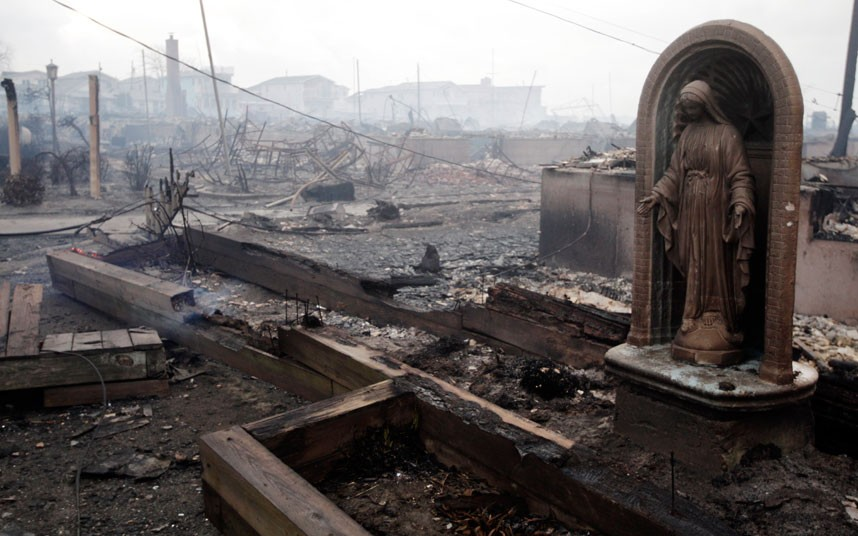
\includegraphics[width=\linewidth]{images/real_example.jpg}
        \caption{Recovering From Sandy: Breezy Point, Queens; Santiago, Cuba}
        \label{fig:real}
    \end{subfigure}
    \hfill % separation between the subfigures
    \begin{subfigure}[b]{0.45\textwidth}
        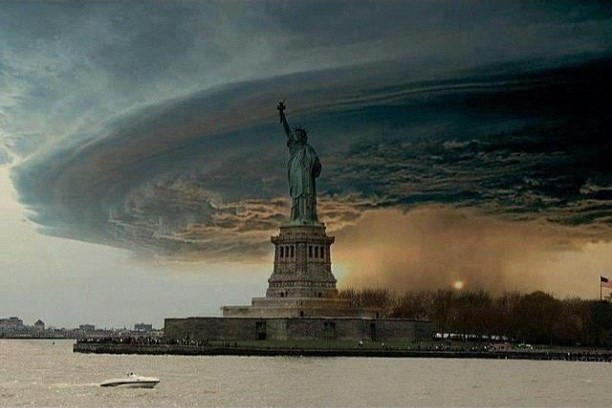
\includegraphics[width=\linewidth]{images/fake_example.jpg}
        \caption{New York gonna be screwed \#sandy \#hurricane \#newyork \#fucked}
        \label{fig:fake}
    \end{subfigure}
    \bigskip 
    \centering
    \begin{subfigure}[b]{0.45\textwidth}
        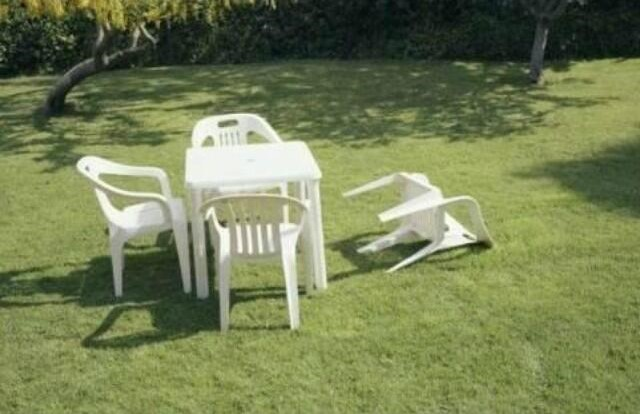
\includegraphics[width=\linewidth]{images/humor_example.jpg}
        \caption{Britain's last hurricane was devastating...}
        \label{fig:humor}
    \end{subfigure}
    \caption{当研究で扱う3カテゴリの投稿例: (a)正しいニュース,(b)フェイクニュース,(c)ジョークニュース}
    \label{fig:examples}
\end{figure}

いずれも2012年に発生したハリケーン・サンディに関してTwitter上で投稿されたものであった.
図\ref{fig:real}では被害を免れた聖母マリア像を写したもので,実際にキューバで撮影されたものであった.
図\ref{fig:fake}ではニューヨークを撮った写真のように見えるが,
元々は2004年に撮影された写真に自由の女神を合成させた写真であった点が指摘された\cite{harmanci_2012}.
図\ref{fig:humor}ではハリケーン・サンディに関連してイギリスにハリケーンが来ないことを茶化すものである.

%
\section{達成目標}
当研究では,上記対象を正確に3カテゴリへ分類するモデルを構築することを目標としている.
具体的には,入力として画像と文章を持ち,それに対してどのカテゴリが該当するかを出力するモデルとなる.
ジョークニュースとフェイクニュースを完全に区別することで,
センセーショナリズムによる影響を最小限に留め,
なおかつ高い精度を維持することを目指すことにする.

当研究を更に発展させると,SNS上でフェイクニュースに該当する記事に対してユーザへ警告を出したり,
ジョーク記事の場合はそれを知らせる追加情報を与えたりするユーザエージェントを開発することへ繋げられる.
また繰り返しフェイクニュースを発信するユーザがいる場合は,
運営側へアカウント停止等のペナルティを迅速に進言するエージェント開発にも発展可能である.

%